%% Le lingue utilizzate, che verranno passate come opzioni al pacchetto babel. Come sempre, l'ultima indicata sar� quella primaria.
%% Se si utilizzano una o pi� lingue diverse da "italian" o "english", leggere le istruzioni in fondo.
\def\thudbabelopt{english,italian}
%% Valori ammessi per target: bach (tesi triennale), mst (tesi magistrale), phd (tesi di dottorato).
%% Valori ammessi per aauheader: '' (vuoto -> nessun header Alpen Adria Univeristat), aics (Department of Artificial Intelligence and Cybersecurity), informatics (Department of Informatics Systems). Il nome del dipartimento � allineato con la versione inglese del logo UniUD.
\documentclass[target=bach,aauheader=]{thud}

%% --- Informazioni sulla tesi ---
%% Per tutti i tipi di tesi
% Scommentare quello di interesse, o mettete quello che vi pare
\course{Informatica}
%\course{Internet of Things, Big Data e Web}
%\course{Matematica}
%\course{Comunicazione Multimediale e Tecnologie dell'Informazione}
\title{Interfacce utente per la selezione \\ di item nel contesto di video giochi \\ in realtà virtuale immersiva}
\author{Paolo Casagrande}
\supervisor{Dott.\ Fabio Buttussi}
%\cosupervisor{Arch.\ Rambaldo Melandri \and Dott.\ Giorgio Perozzi}
%\tutor{Guido Necchi}
%% Campi obbligatori: \title, \author e \course.
%% Altri campi disponibili: \reviewer, \tutor, \chair, \date (anno accademico, calcolato in automatico), \rights
%% Con \supervisor, \cosupervisor, \reviewer e \tutor si possono indicare pi� nomi separati da \and.
%% Per le sole tesi di dottorato:
%\phdnumber{313}
%\cycle{XXVIII}
%\contacts{Via della Sintassi Astratta, 0/1\\65536 Gigatera --- Italia\\+39 0123 456789\\\texttt{http://www.example.com}\\\texttt{inbox@example.com}}

%% --- Pacchetti consigliati ---
%% pdfx: per generare il PDF/A per l'archiviazione. Necessario solo per la versione finale
\usepackage[a-1b]{pdfx}
%% hyperref: Regola le impostazioni della creazione del PDF... pi� tante altre cose. Ricordarsi di usare l'opzione pdfa.
\usepackage[pdfa]{hyperref}
%% tocbibind: Inserisce nell'indice anche la lista delle figure, la bibliografia, ecc.

%% --- Stili di pagina disponibili (comando \pagestyle) ---
%% sfbig (predefinito): Apertura delle parti e dei capitoli col numero grande; titoli delle parti e dei capitoli e intestazioni di pagina in sans serif.
%% big: Come "sfbig", solo serif.
%% plain: Apertura delle parti e dei capitoli tradizionali di LaTeX; intestazioni di pagina come "big".

% package per le immagini
\usepackage{graphicx}
\graphicspath{ {./images/} }

\begin{document}
\maketitle

%% Dedica (opzionale)
%\begin{dedication}
%	Al mio cane,\par per avermi ascoltato mentre ripassavo le lezioni.
%\end{dedication}

%% Ringraziamenti (opzionali)
\acknowledgements
Speriamo bene
%% Sommario (opzionale)
%\abstract
%Nunc ac dignissim ipsum, quis pulvinar elit. Mauris congue nec leo ornare lobortis. Nulla hendrerit pretium diam nec lobortis. Nullam aliquam laoreet nisl, sit amet facilisis lectus accumsan ut. Duis et elit hendrerit metus venenatis condimentum. Integer id eros molestie, interdum leo sit amet, aliquet metus. Integer fermentum tristique magna, vel luctus neque rhoncus vel. Ut hendrerit et quam et semper. Mauris egestas, odio sed aliquet luctus, magna orci euismod odio, vitae lacinia tellus tellus non lectus. Aliquam urna neque, porta et mattis aliquam, congue sit amet lorem. In ultrices augue sit amet ante vehicula, vitae rhoncus turpis auctor. Donec porta scelerisque eros, at mollis enim imperdiet ut. 

%% Indice
\tableofcontents

%% Lista delle tabelle (se presenti)
%\listoftables

%% Lista delle figure (se presenti)
\listoffigures

%% Corpo principale del documento
\mainmatter

%% Parte
%% La suddivisione in parti � opzionale; solitamente sono sufficienti i capitoli.
%\part{Parte}
%\nocite{*} %% rimuovere magari in seguito
%% Capitolo
\chapter{Introduzione} % Introduzione alla VR + Intro dispositivi + Intro capitoli
\label{intro}
La Realtà Virtuale (Virtual Reality, VR) è un'interfaccia avanzata uomo-computer che simula un ambiente realistico \cite{Zheng}.
All'interno di questo ambiente l'utente è libero di muoversi, esplorare ed interagire con qualsiasi cosa, alimentando la sensazione di sentirsi effettivamente presente all'interno di un mondo virtuale.
Al giorno d'oggi, la Realtà Virtuale può essere applicata a vari settori tra cui l'intrattenimento, l'educazione, medico e commerciale. \\

L'interazione tra uomo e ambiente virtuale avviene attraverso specifici dispositivi.
L'interfaccia avanzata più utilizzata nella Realtà Virtuale è il visore VR. 
Questo visore, denominato Head Mounted Dispaly, può essere indossato come un casco che mostra all'utente il mondo virtuale a 360°.
Il visore VR utilizzato per l'esperimento è il Visore VR HTC Vive Pro, visibile in figura \ref{fig:vive_pro}.

\begin{figure}[h]
    \centering
    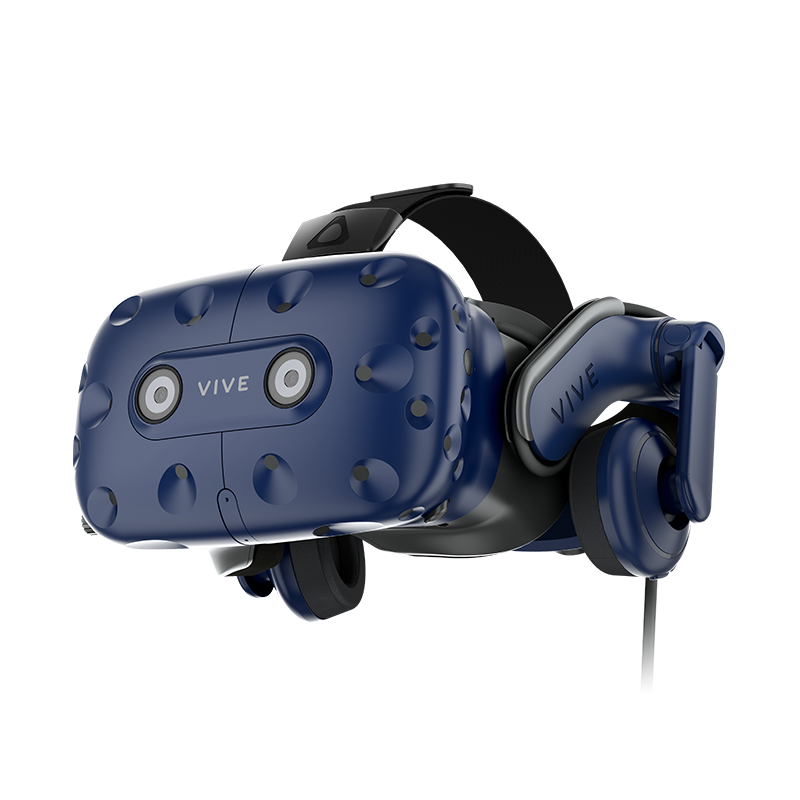
\includegraphics[width=0.25\textwidth]{vive_pro}
    \caption{Visore VR HTC Vive Pro}
    \label{fig:vive_pro}
\end{figure}

Insieme al visore, per interagire all'interno dell'ambiente virtuale, l'utente utilizza una coppia di controller per muovere entrambe le mani \ref{fig:vive_contr}.
Questi controller mappano il movimento delle mani nello spazio reale, che viene poi rappresentato nel mondo virtuale. 
L'utente può premere i tasti sui controller per esercitare azioni specifiche che interagiscono con l'ambiente virtuale. \\

\begin{figure}[h]
    \centering
    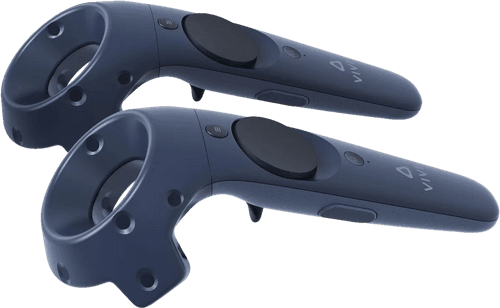
\includegraphics[width=0.25\textwidth]{vive_contr}
    \caption{Controller per HTC Vive Pro}
    \label{fig:vive_contr}
\end{figure}

\newpage
L'obiettivo della tesi è quello di sviluppare un'interfaccia virtuale efficace che permetta agli utenti di selezionare determinati item.
L'efficacia dell'interfaccia dipenderà dalla facilità di selezione di un item, dalla rapidità con la quale lo si seleziona e dalla fatica che bisogna fare per selezionarlo.
Sono state progettate molte interfacce, come verrà spiegato meglio nei prossimi capitoli, per ottenere le due interfacce finali migliori. \\


Nel capitolo 2 viene descritto lo stato dell'arte riguardante la Realtà Virtuale e alcuni studi riguardo a interfacce in ambienti virtuali.
Nel capitolo 3 si spiega la programmazione dell'ambiente virtuale, nel capitolo 4 come sono state progettate tutte le interfacce.
Nel capitolo 5 vengono poi confrontate le interfacce più efficaci, mentre nel capitolo 6 si conclude la tesi parlando di ulteriori sviluppi futuri.
%% Sezione
%\section{Titolo della Sezione}

%% Sottosezione
%\subsection{Sottosezione}

\chapter{Stato dell'arte} % Studi VR e interfacce + Legame tra VR e dispositivi
\section{VR immersiva e UI}
L'Interfaccia Utente (User Interface, UI) permette l'interazione tra uomo e macchina.
Si possono implementare quattro interfacce diverse all'interno di :
\begin{itemize}
    \item Diegetica: l'UI è integrata all'interno dell'ambiente virtuale, ad esempio fondendosi con oggetti che ne fanno parte;
    \item Non-diegetica: l'UI viene mostrata fuori dal mondo virtuale, in sovrimpressione sullo schermo;
    \item Meta: sono interfacce 2D rappresentate nel mondo 3D che fanno parte del mondo virtuale;
    \item Spaziale: sono elementi UI 3D che non fanno parte del mondo virtuale e servono solo all'utente come informazione;
\end{itemize} 

Esistono molti studi che comparano diverse interfacce per interagire nelle applicazioni VR immersive.
Ad esempio, uno studio condotto da Daniel Hepperle et al.\cite{Hepperle} ha confrontato tre diverse interfacce - 2D, 3D e a comando vocale - per capire quale fosse la migliore per la Realtà Virtuale.  
Nello studio sono stati coinvolti 30 partecipanti, di cui 20 maschi e 10 femmine.
Degli utenti, solo il 66\% aveva esperienza con sistemi VR e il 50\% aveva già usato un dispositivo 3D prima d'ora.
La prova consisteva nel completare 17 compiti con le 3 interfacce nel minor tempo possibile e infine compilare un questionario.
I compiti comprendevano selezione, manipolazione, creazione, rotazione e modifica di oggetti virtuali.
Dai risultati è emerso che gli utenti, usando l'interfaccia sviluppata in 3D, consideravano l'input intuitivo e naturale; inoltre, rispetto alle altre interfacce, si sentivano più immersi nell'attività. \\

Uno studio di Rennan Raffaele et al.\cite{Raffaele} ha analizzato quale interfaccia immersiva fosse la migliore nei giochi VR.
Le interfacce a confronto proponevano rappresentazione spaziale, meta, diegetica e non-diegetica.
Allo studio hanno partecipato 50 utenti, che spaziavano tra designer, sviluppatori e videogiocatori.
I partecipanti dovevano infine compilare un questionario che paragonava 16 interfacce diverse utilizzate nei videogiochi.
I risultati hanno mostrato che la rappresentazione diegetica è quella che permette la maggiore immersività di un'interfaccia in un ambiente virtuale.

Quentin Marre et al. \cite{Marre} hanno voluto testare quale interfaccia, tra non-diegetica e diegetica, fosse la migliore in un videogioco sparatutto.
Le informazioni sulla salute e munizioni dell'arma erano nel primo caso sovrapposti nello schermo, mentre nel secondo erano integrati nel mondo virtuale.
In questo studio sono stati coinvolti 41 partecipanti, composti da giocatori esperti e inesperti. 
Questa ricerca ha concluso che un'UI diegetica ha avuto un effetto positivo sulla performance degli utenti.
Questo studio conclude consigliando ai lettori di usare interfacce integrate il più possibile con il mondo virtuale.

La tesi si concentra dunque sullo sviluppo di interfacce per la selezione di item, partendo da soluzioni semplici e procedendo verso soluzioni sempre più immersive. 

\chapter{Progettazione dell'ambiente virtuale} % Spiegazione livello e menu vari + periferiche

\section{Periferiche utilizzate}
Per l'obiettivo di questa tesi sono state utilizzate le periferiche approfondite in seguito.

\subsection{Pedana KAT WALK Mini S}
Quando si utilizza un visore VR le possibilità per il movimento nell'ambiente sono due: spostarsi tramite teletrasporto o camminare nello spazio reale.
Usando il teletrasporto ci si sposta premento un tasto sul controller VR e rimanendo fermi nella realtà, il che può attenuare il senso di immersione in un ambiente virtuale.
Per muoversi nel mondo reale, invece, bisogna avere a disposizione uno spazio ampio, altrimenti il rischio è di andare a sbattere da qualche parte senza vedere dove si va.
Una soluzione che permette di camminare nello spazio virtuale senza spostarsi realmente è la Pedana KAT WALK Mini S \ref{fig:kat_walk}.
Questa permette di spostarsi a 360° nel mondo virtuale, di correre, saltare e accovacciarsi. 
Bisogna indossare delle coperture sulla suola delle scarpe per creare l'effetto di pattinamento sulla pedana.    

\begin{figure}[h]
    \centering
    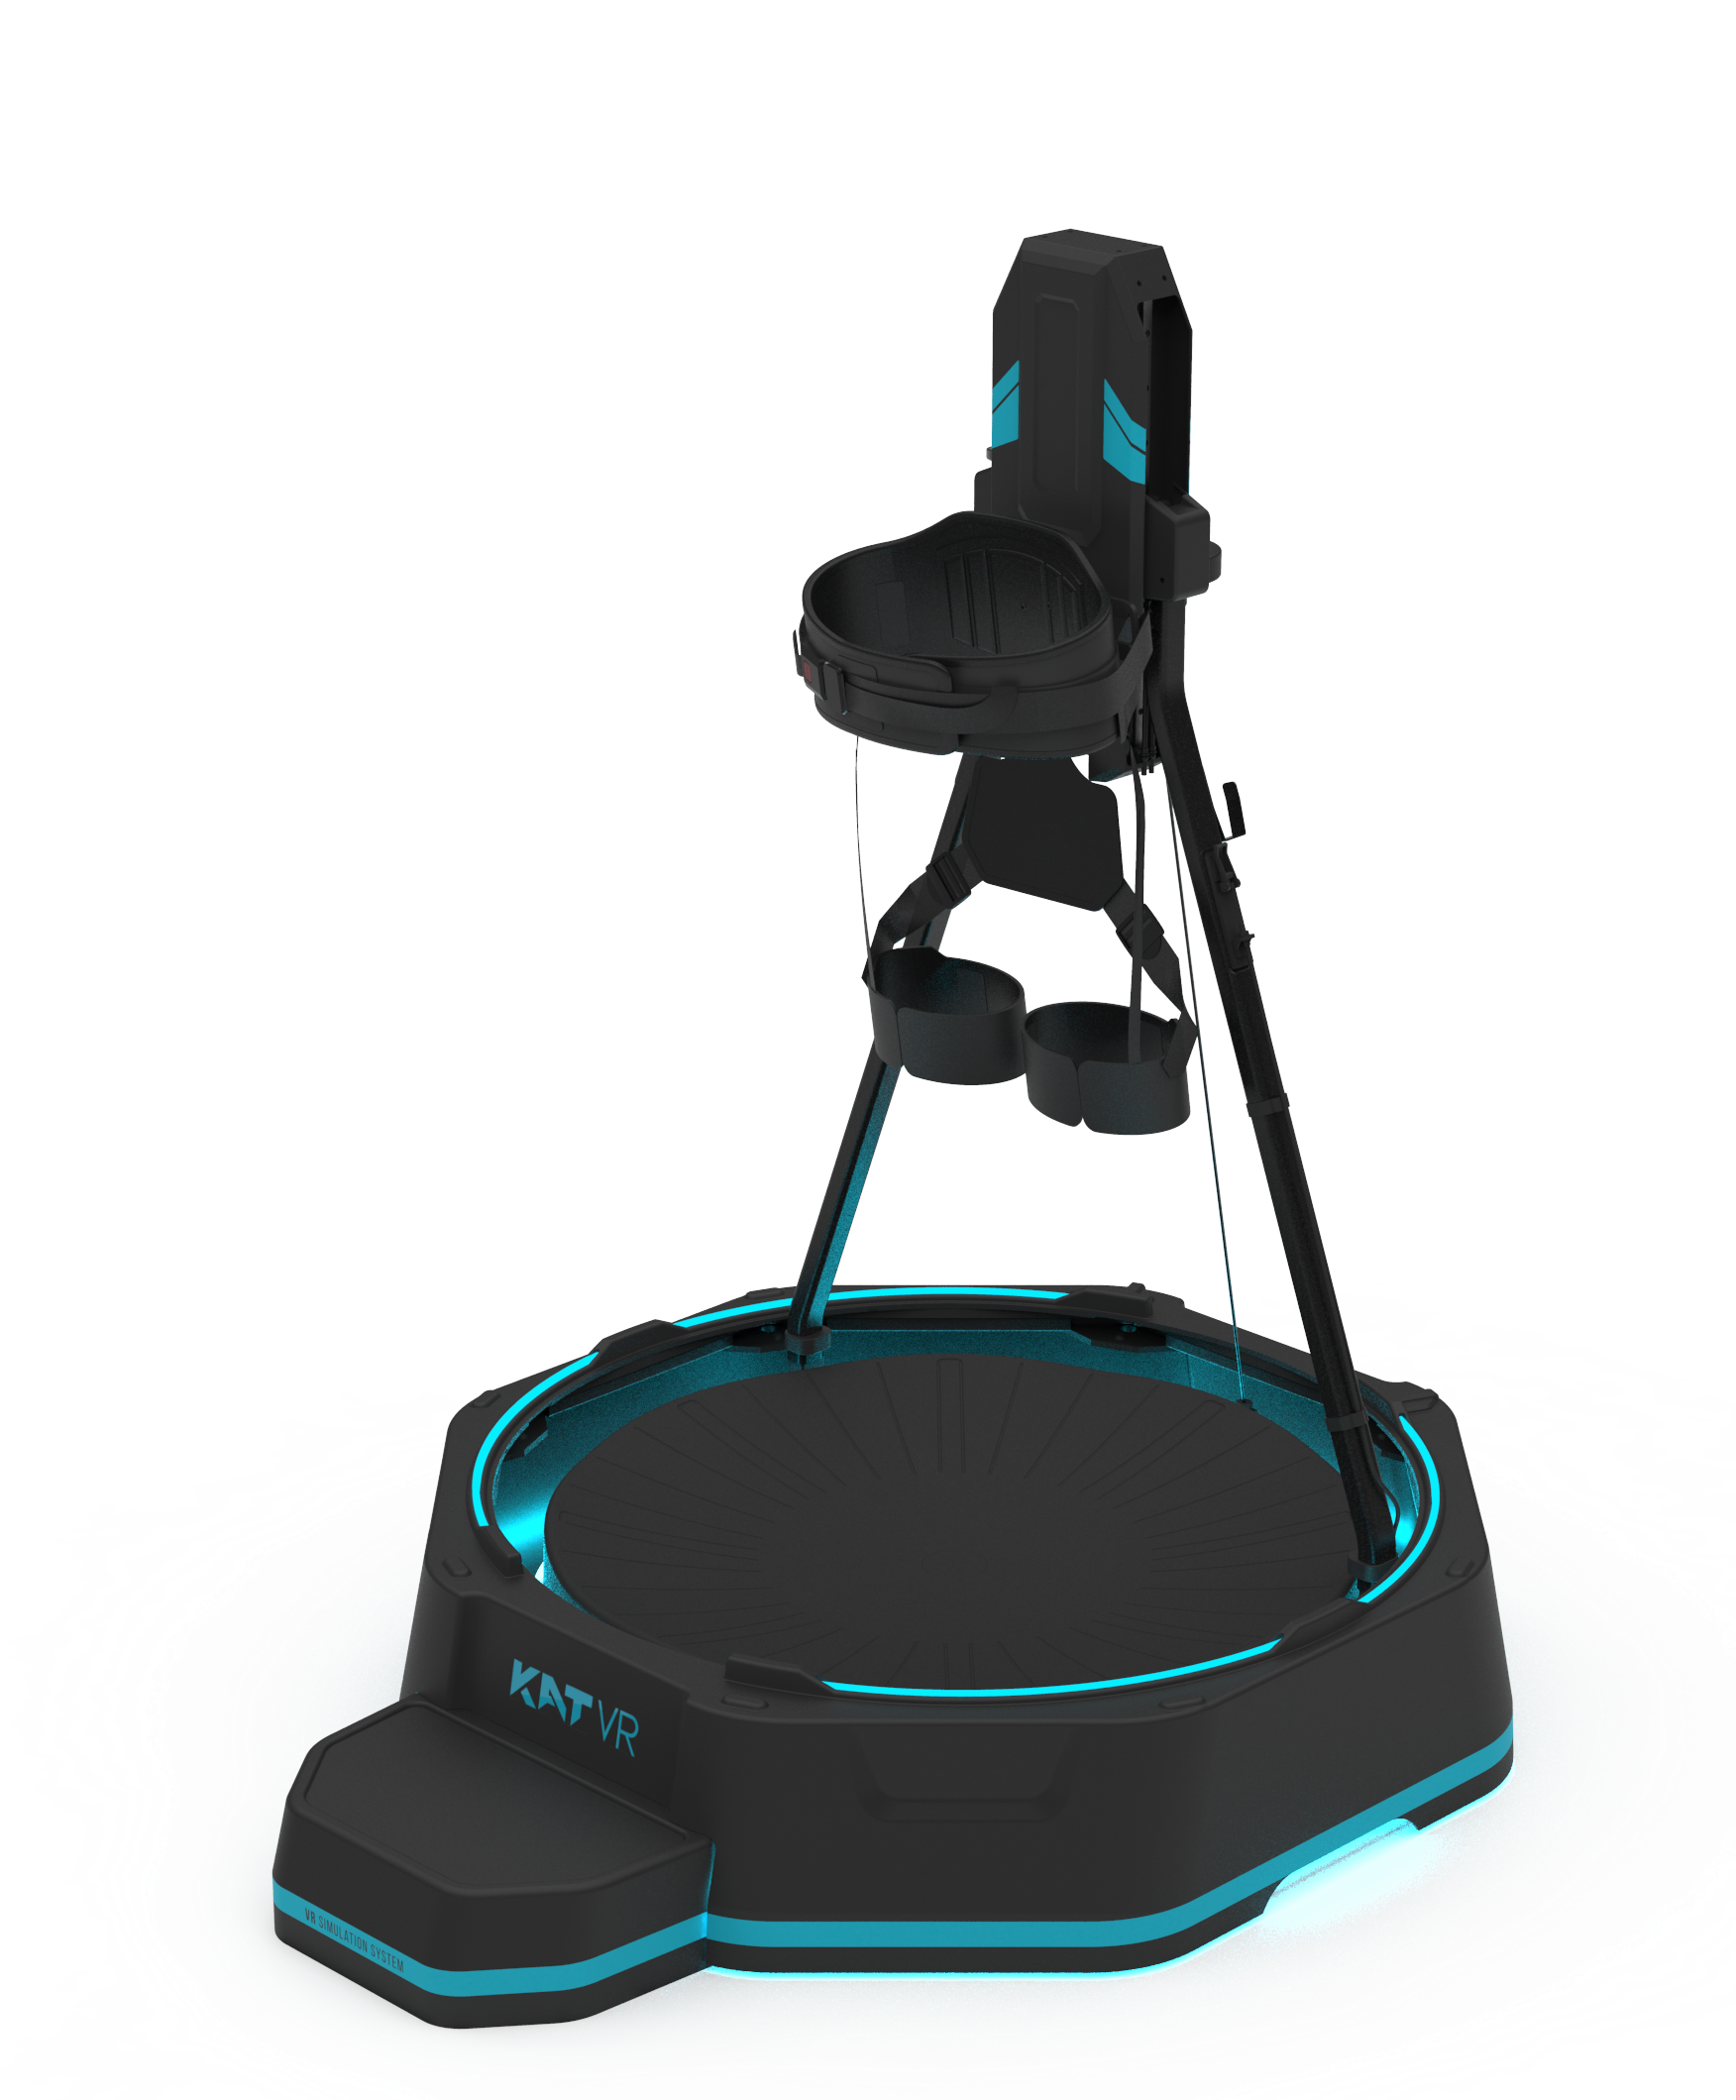
\includegraphics[width=0.30\textwidth]{kat_walk_mini}
    \caption{Pedana KAT WLK Mini S}
    \label{fig:kat_walk}
\end{figure}

\subsection{Visore e controller VR}
Come anticipato nella Sezione \ref{intro}, sono stati utlizzati il visore HTC Vive Pro e i suoi controller.
Inoltre, per poter mappare l'ambiente reale e tenere traccia della posizione di ogni dispositivo, sono state utilizzate anche le telecamere SteamVR Base Station.

\section{Software Utilizzati}
Per programmare un ambiente virtuale interagibile tramite visore VR e pedana KAT WALK è stato utilizzato il game engine Unity.
Per potersi interfacciare con la pedana e calibrarla è stato usato il KATVR SDK, un plug-in sviluppato appositamente da KATVR.
Le icone delle chiavi sono state generate usando il plug-in di Unity “ThumbCreator” di AndreaDev3D.
Infine, il plug-in OpenXR ha permesso a unity di interfacciarsi con il visore HTC Vive Pro.

\section{Menu Iniziale}
\label{menu_init}
All'apertura dell'applicazione si può scegliere, dal menu iniziale, una delle 4 voci:
\begin{itemize}
    \item Calibrazione Pedana: serve per calibrare la pedana in modo da spostarsi correttamente nell'ambiente virtuale;
    \item Test Pedana: fa provare la pedana attraverso un tutorial, spiegato in seguito \ref{tut_ped};
    \item Primo Menu e Secondo Menu: entrambe fanno provare un menu specifico, spiegato in seguito \ref{menu_int};
\end{itemize} 
Inoltre, l'intera attività può essere terminata premendo sulla "X" rossa in alto a destra.

\begin{figure}[h]
    \centering
    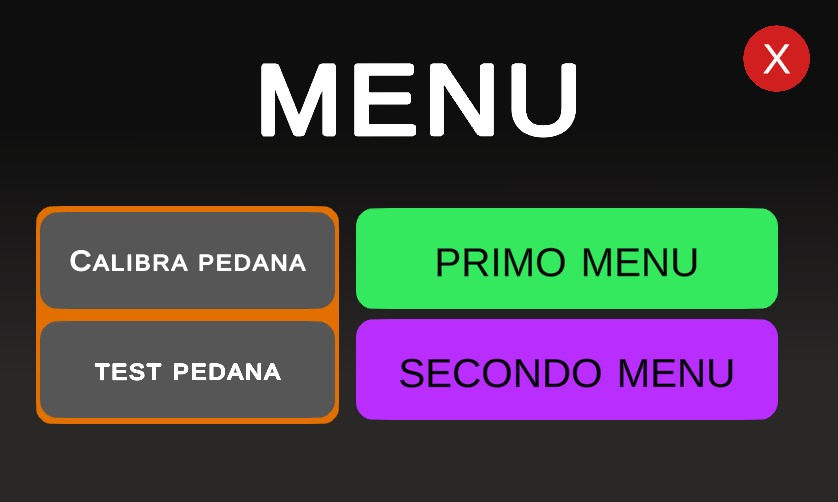
\includegraphics[width=0.40\textwidth]{menu_screen}
    \caption{Schermata del Menu Iniziale}
    \label{fig:menu_screen}
\end{figure}

\subsection{Sottomenu delle Interfacce}
\label{menu_int}
Dal Menu Iniziale si può scegliere quale delle due interfacce testare.
Questa schermata presenta:
\begin{itemize}
    \item Tutorial: si può provare l'interfaccia senza fare il livello, spiegata in seguito \ref{tut_int};
    \item Gioca: si può accedere al livello, spiegato nel dettaglio alla sezione \ref{level};
\end{itemize}
Inoltre è presente una freccia in alto a destra che permette di tornare alla schermata precedente, ovvero il Menu Iniziale \ref{menu_init}.

\begin{figure}[h]
    \centering
    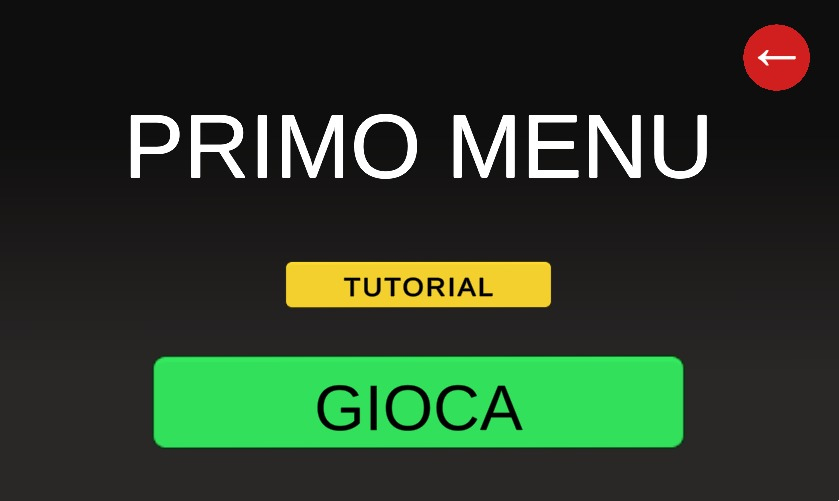
\includegraphics[width=0.40\textwidth]{first_menu}
    \caption{Schermata del Menu della Prima Interfaccia}
    \label{fig:first_menu}
\end{figure}

\section{Tutorial Design}
Pensando a questo progetto come una risorsa per eventuali test futuri su utenti, sono stati implementati due tipi di tutorial.

\subsection{Tutorial per la pedana}
\label{tut_ped}
Dal Menu Iniziale \ref{menu_init} si può accedere a un tutorial per l'utilizzo della pedana.
Questo tutorial permette all'utente di muoversi in un ambiente chiuso e piatto.
L'utente può seguire dei tracciati tratteggiati posti sul terreno per acquisire familiarità con la pedana.
Inoltre nell'ambiente circostante sono stati posizionati degli oggetti 3D immobili e solidi per dare qualche punto di riferimento in più all'utente. 

\subsection{Tutorial per le interfacce}
\label{tut_int}
All'interno del Menu di ogni interfaccia \ref{menu_int} si può testare l'interfaccia scelta.
Le due interfacce sono i risultati dello sviluppo del progetto e all'interno del tutorial si può provarle con calma al fine di comprenderle al meglio.
Il tutorial presenta una struttura simile al livello ma senza alcune componenti, dunque le differenze verranno approfondite più avanti \ref{level}. 

\section{Level Design}
\label{level}



\section{Chiavi e porte}


\chapter{Design delle interfacce} % Percorso per arrivare alle interfacce adatte


\section{Interfaccia Select} % < O >

\section{Interfaccia Pie} % a torta

\section{Interfaccia Swish} % bisogna indicare, scomodo

\section{Interfaccia Spin} % ruotare ad ogni chiave a destra o sinistra, evoluzione di select ma con rotazione polso

\section{Interfaccia Wrist Rotation} % rotazione con menu a U

\section{Interfaccia Finale 1: Wrist-Spin} % fusione -> punti di forza di entrambi
\label{int_wrist-spin}


\section{Interfaccia Finale 2: Socket Menu} % socket nelle mani a U
\label{int_socket}



\chapter{Discussione}
Analisi dei due menu finali?


\chapter{Conclusioni} % cosa si può fare
Studio con utenti, questionari da poter applicare, dati raccoglibili

%% Fine dei capitoli normali, inizio dei capitoli-appendice (opzionali)
%\appendix
%\part{Appendici}
%\chapter{Titolo della prima appendice}

%% Parte conclusiva del documento; tipicamente per riassunto, bibliografia e/o indice analitico.
\backmatter

%% Riassunto (opzionale)
%\summary
%Maecenas tempor elit sed arcu commodo, dapibus sagittis leo egestas. Praesent at ultrices urna. Integer et nibh in augue mollis facilisis sit amet eget magna. Fusce at porttitor sapien. Phasellus imperdiet, felis et molestie vulputate, mauris sapien tincidunt justo, in lacinia velit nisi nec ipsum. Duis elementum pharetra lorem, ut pellentesque nulla congue et. Sed eu venenatis tellus, pharetra cursus felis. Sed et luctus nunc. Aenean commodo, neque a aliquam bibendum, mauris augue fringilla justo, et scelerisque odio mi sit amet diam. Nulla at placerat nibh, nec rutrum urna. Donec ut egestas magna. Aliquam erat volutpat. Phasellus vestibulum justo sed purus mattis, vitae lacinia magna viverra. Nulla rutrum diam dui, vel semper mi mattis ac. Vestibulum ante ipsum primis in faucibus orci luctus et ultrices posuere cubilia Curae; Donec id vestibulum lectus, eget tristique est.

%% Bibliografia (praticamente obbligatoria)
\bibliographystyle{plain_\languagename}%% Carica l'omonimo file .bst, dove \languagename � la lingua attiva.
%% Nel caso in cui si usi un file .bib (consigliato)
\bibliography{thud}
%% Nel caso di bibliografia manuale, usare l'environment thebibliography.

%% Per l'indice analitico, usare il pacchetto makeidx (o analogo).

\end{document}

--- Istruzioni per l'aggiunta di nuove lingue ---
Per ogni nuova lingua utilizzata aggiungere nel preambolo il seguente spezzone:
    \addto\captionsitalian{%
        \def\abstractname{Sommario}%
        \def\acknowledgementsname{Ringraziamenti}%
        \def\authorcontactsname{Contatti dell'autore}%
        \def\candidatename{Candidato}%
        \def\chairname{Direttore}%
        \def\conclusionsname{Conclusioni}%
        \def\cosupervisorname{Co-relatore}%
        \def\cosupervisorsname{Co-relatori}%
        \def\cyclename{Ciclo}%
        \def\datename{Anno accademico}%
        \def\indexname{Indice analitico}%
        \def\institutecontactsname{Contatti dell'Istituto}%
        \def\introductionname{Introduzione}%
        \def\prefacename{Prefazione}%
        \def\reviewername{Controrelatore}%
        \def\reviewersname{Controrelatori}%
        %% Anno accademico
        \def\shortdatename{A.A.}%
        \def\summaryname{Riassunto}%
        \def\supervisorname{Relatore}%
        \def\supervisorsname{Relatori}%
        \def\thesisname{Tesi di \expandafter\ifcase\csname thud@target\endcsname Laurea\or Laurea Magistrale\or Dottorato\fi}%
        \def\tutorname{Tutor aziendale}%
        \def\tutorsname{Tutor aziendali}%
    }
sostituendo a "italian" (nella 1a riga) il nome della lingua e traducendo le varie voci.